% pipeline_v4 (fig:pipeline, figure*): one keyframe update of the UAGS field. The two rows of v2
% (evidence on top, change handling below) with the key equation of every block, drawn in the
% style of v3 (short titles, larger pictures, colour per role): v2 had a paragraph per box, v3 had
% no equations (user, 2026-11-02: "pipeline_v3 is quite basic ... improve by using pipeline_v2;
% add some other equation and block"). v2 and v3 are kept. Notation follows Sec. III of main.tex
% (the index n of a Gaussian is dropped except in w_{p,n} and f_n). Thumbnails (validation scenes
% only) as v2, made by scripts/render_pipeline_thumbs.py: Replica office_0 mapping keyframe 825;
% NeRF-Object-Removal 002, update view 335 (reset Gaussians in orange) and its mapping-pass null.
% Build (from papers/): pdflatex -output-directory <dir> figs/pipeline_v4.tex
% Natural width = 7.16 in (IEEEtran journal \textwidth): titles print at 8 pt, the rest at 7 pt,
% small notes at 6 pt.
\documentclass[tikz,border=1pt]{standalone}
\usepackage[T1]{fontenc}
\renewcommand{\rmdefault}{ptm}          % Times text, CM math: as the paper (IEEEtran)
\usepackage{amsmath,amssymb}
\usepackage{graphicx}
\graphicspath{{figs/pipeline_thumbs/}{pipeline_thumbs/}}
\usetikzlibrary{arrows.meta,calc}

\newcommand{\R}{\mathbf{R}}
\newcommand{\zv}{\mathbf{z}}
\newcommand{\uv}{\mathbf{u}}
\newcommand{\fv}{\mathbf{f}}
\newcommand{\Fv}{\mathbf{F}}
\newcommand{\Yv}{\mathbf{Y}}
\newcommand{\tv}{\mathbf{t}}
\newcommand{\muv}{\boldsymbol{\mu}}
\newcommand{\Sph}{\mathbb{S}}
\newcommand{\old}{\mathrm{old}}
\newcommand{\new}{\mathrm{new}}
\newcommand{\epi}{\mathrm{epi}}
\newcommand{\ale}{\mathrm{ale}}
\newcommand{\sixpt}{\fontsize{6}{7}\selectfont}

% Okabe-Ito, as the teaser: evidence blue, change orange, read-out green
\definecolor{okblue}{HTML}{0072B2}
\definecolor{okorange}{HTML}{E69F00}
\definecolor{okgreen}{HTML}{009E73}
\colorlet{evid}{okblue}
\colorlet{evidtxt}{okblue!85!black}
\colorlet{chg}{okorange!85!black}
\colorlet{chgtxt}{okorange!50!black}
\colorlet{rd}{okgreen!80!black}
\colorlet{rdtxt}{okgreen!55!black}

% generated legend colours / names and the threshold position (render_pipeline_thumbs.py compose)
\InputIfFileExists{figs/pipeline_thumbs/values.tex}{}{% generated by scripts/render_pipeline_thumbs.py compose; do not edit
\definecolor{labA}{rgb}{0.1216,0.4667,0.7059}
\newcommand{\labnameA}{wall}
\definecolor{labB}{rgb}{1.0000,0.4980,0.0549}
\newcommand{\labnameB}{ceiling}
\definecolor{labC}{rgb}{0.5490,0.3373,0.2941}
\newcommand{\labnameC}{tv-screen}
\definecolor{labD}{rgb}{0.8392,0.1529,0.1569}
\newcommand{\labnameD}{rug}
\newcommand{\nullthetafrac}{0.6250}
}

% step number: white digit on a disc of the stage colour
\newcommand{\step}[2]{\tikz[baseline=(s.base)]\node[circle,fill=#1,text=white,inner sep=0pt,
  minimum size=3.3mm,font=\scriptsize\bfseries](s){#2};}

\begin{document}
\begin{tikzpicture}[
  x=1cm, y=1cm, font=\scriptsize, line cap=round,
  stage/.style={draw, rounded corners=3pt, line width=0.6pt, anchor=north west},
  evidbox/.style={stage, draw=evid, fill=evid!5},
  chgbox/.style={stage, draw=chg, fill=okorange!8},
  rdbox/.style={stage, draw=rd, fill=okgreen!6},
  ttl/.style={anchor=north west, inner sep=2pt, font=\footnotesize\bfseries},
  tag/.style={anchor=north west, inner sep=1pt, font=\sixpt, text=black!60},
  lbl/.style={align=center, inner sep=1pt},
  img/.style={inner sep=0pt},
  frm/.style={draw=black!60, line width=0.3pt},
  arr/.style={-{Stealth[length=1.8mm,width=1.4mm]}, line width=0.75pt},
  chgarr/.style={arr, draw=chg},
]
% ------------------------------------------------------------------ geometry (cm)
% columns: left edge, width; total 18.19 cm = 7.16 in
\def\xA{0.00}  \def\wA{2.30}           % keyframe (both rows)
\def\xB{2.70}  \def\wB{3.05}           % lifting      | threshold
\def\xC{6.15}  \def\wC{2.55}           % observation  | change test (spans C and D)
\def\xD{9.10}  \def\wD{2.40}           % running sums |
\def\wCD{5.35}                         % change test: from xC to xD+wD
\def\xE{11.90} \def\wE{3.59}           % uncertainty  | reset, re-admission
\def\xF{15.89} \def\wF{2.30}           % read-out (both rows)
\def\hT{3.60}                          % top row: y 0 .. -hT
\def\yB{-4.05} \def\hB{2.35}           % bottom row: top edge, height
\def\hAll{6.40}                        % tall boxes
\def\ya{-1.80}                         % top-row flow arrows

% ================================================================== boxes
\node[stage, draw=black!55, fill=black!3, minimum width=\wA cm, minimum height=\hAll cm] at (\xA,0) {};
\node[evidbox, minimum width=\wB cm, minimum height=\hT cm] at (\xB,0) {};
\node[evidbox, minimum width=\wC cm, minimum height=\hT cm] at (\xC,0) {};
\node[evidbox, minimum width=\wD cm, minimum height=\hT cm] at (\xD,0) {};
\node[evidbox, minimum width=\wE cm, minimum height=\hT cm] at (\xE,0) {};
\node[rdbox,   minimum width=\wF cm, minimum height=\hAll cm] at (\xF,0) {};
\node[chgbox,  minimum width=\wB cm, minimum height=\hB cm] at (\xB,\yB) {};
\node[chgbox,  minimum width=\wCD cm, minimum height=\hB cm] at (\xC,\yB) {};
\node[chgbox,  minimum width=\wE cm, minimum height=\hB cm] at (\xE,\yB) {};

% ================================================================== (1) keyframe and LSeg features
\node[ttl] at (\xA,0) {\step{black!75}{1} Keyframe};
\def\tw{2.05} \def\th{1.5375}          % 4:3
\node[img, anchor=north] (rgb) at (\xA+\wA/2, -0.60) {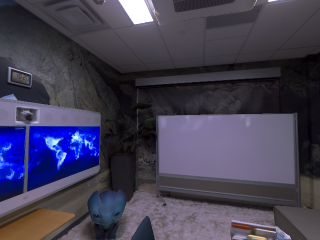
\includegraphics[width=\tw cm,height=\th cm]{keyframe_rgb.png}};
\draw[frm] (rgb.south west) rectangle (rgb.north east);
\node[lbl, anchor=south west, fill=white, fill opacity=0.8, text opacity=1, inner sep=1.2pt] at (rgb.south west) {RGB(-D)};
\node[img, anchor=north] (pca) at (\xA+\wA/2, -2.85) {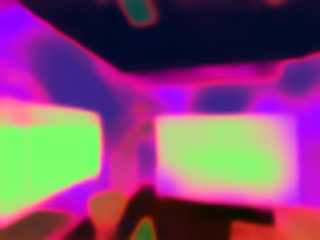
\includegraphics[width=\tw cm,height=\th cm]{features_pca.png}};
\draw[frm] (pca.south west) rectangle (pca.north east);
\draw[arr, black!70] (rgb.south) -- (pca.north) node[midway, right=1pt, lbl] {LSeg};
\node[lbl, anchor=north] at (pca.south) {$\zv_p\in\Sph^{d-1}$\\[1pt] PCA, $d{=}64$};

% ================================================================== (2) lifting: one render + one backward
\node[ttl, text=evidtxt] at (\xB,0) {\step{evid}{2} Lifting};
\begin{scope}[shift={(\xB+0.42, -0.98)}, scale=0.78]
  \draw[black!75, line width=0.5pt, fill=white] (-0.16,-0.20) rectangle (0.10,0.20);
  \draw[black!75, line width=0.5pt, fill=black!10] (0.10,-0.12) -- (0.32,-0.32) -- (0.32,0.32) -- (0.10,0.12) -- cycle;
  \foreach \yy in {0.45,0.02,-0.42}
    \draw[evid!55, line width=0.4pt, dash pattern=on 1.2pt off 1pt] (0.32,0) -- (1.70,\yy);
  \draw[fill=black!12, draw=black!40, line width=0.3pt, rotate around={30:(2.15,0.48)}]  (2.15,0.48) ellipse (0.34 and 0.13);
  \draw[fill=black!12, draw=black!40, line width=0.3pt, rotate around={-25:(2.25,-0.45)}] (2.25,-0.45) ellipse (0.30 and 0.12);
  \draw[fill=black!12, draw=black!40, line width=0.3pt, rotate around={70:(1.75,-0.05)}] (1.75,-0.05) ellipse (0.26 and 0.10);
  \draw[fill=evid!45, draw=evid!80!black, line width=0.45pt, rotate around={-10:(2.12,0.04)}] (2.12,0.04) ellipse (0.36 and 0.15);
\end{scope}
\node[lbl] at (\xB+\wB/2, -1.66) {one render $+$ one backward};
\node[lbl] at (\xB+\wB/2, -2.06) {$\Fv_p=\sum_n w_{p,n}\fv_n$};
\node[lbl] at (\xB+\wB/2, -2.47) {$\partial_{\fv_n}\!\sum_p\Yv_p^{\!\top}\Fv_p$};
\node[lbl] at (\xB+\wB/2, -2.83) {${}=\sum_p w_{p,n}\Yv_p$};
\node[lbl, text=evidtxt] at (\xB+\wB/2, -3.25) {$\Rightarrow$\ $\R_v$,\ $m_v$ per Gaussian};

% ================================================================== (3) one observation per view
\node[ttl, text=evidtxt] at (\xC,0) {\step{evid}{3} Observation};
\begin{scope}[shift={(\xC+\wC/2, -1.30)}]
  \draw[black!40, line width=0.4pt] (0,0) circle (0.52);
  \foreach \a in {14,30,46,60,74,112} \draw[-{Stealth[length=1.0mm]}, black!45, line width=0.35pt] (0,0) -- (\a:0.52);
  \draw[-{Stealth[length=1.6mm]}, evid, line width=1.1pt] (0,0) -- (52:0.40);
  \node[lbl, text=black!60, anchor=west] at (8:0.54) {$\zv_p$};
  \node[lbl, text=evidtxt, anchor=east] at (205:0.10) {$\uv_v$};
\end{scope}
\node[lbl] at (\xC+\wC/2, -2.25) {$\uv_v=\R_v/m_v$};
\node[lbl, font=\sixpt] at (\xC+\wC/2, -2.75) {$\omega_v=\min\!\big(1,\tfrac{m_v}{a_0HW}\big)$};
\node[lbl, font=\sixpt, text=black!60] at (\xC+\wC/2, -3.25) {one per view and Gaussian};

% ================================================================== (4) running sums
\node[ttl, text=evidtxt] at (\xD,0) {\step{evid}{4} Running sums};
\node[lbl, align=left, anchor=north] at (\xD+\wD/2, -0.58)
  {$\R=\sum\omega\,\uv$\\[2.5pt] $s=W_1=\sum\omega$\\[2.5pt] $W_2=\sum\omega^2$\\[2.5pt] $Q=\sum\omega^2\lVert\uv\rVert^2$};
\node[lbl, text=chgtxt] at (\xD+\wD/2, -3.05) {buckets $\R^{\old}$, $\R^{\new}$};

% ================================================================== (5) vMF posterior and two uncertainties
\node[ttl, text=evidtxt] at (\xE,0) {\step{evid}{5} Two uncertainties};
\node[lbl] at (\xE+\wE/2, -0.66) {vMF:\ $\muv^\star=\R/\lVert\R\rVert$};
\def\uw{1.68} \def\uh{1.26}            % 4:3
\node[img, anchor=north west] (ue) at (\xE+0.08, -0.95) {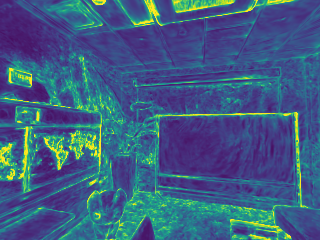
\includegraphics[width=\uw cm,height=\uh cm]{u_epi.png}};
\draw[frm] (ue.south west) rectangle (ue.north east);
\node[img, anchor=north east] (ua) at (\xE+\wE-0.08, -0.95) {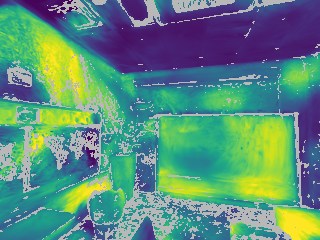
\includegraphics[width=\uw cm,height=\uh cm]{u_ale.png}};
\draw[frm] (ua.south west) rectangle (ua.north east);
\node[lbl, anchor=south east, fill=white, fill opacity=0.8, text opacity=1, inner sep=0.8pt, font=\sixpt] at (ua.south east) {grey: $s<\tau_{\min}$};
\node[lbl, anchor=north] at (ue.south) {$u^{\epi}=\tfrac{1}{1+s}$};
\node[lbl, anchor=north] at (ua.south) {$u^{\ale}=1-\hat\rho$};
\node[lbl] at (\xE+\wE/2, -3.08) {$\hat\rho^{\,2}=\Big[\dfrac{\lVert\R\rVert^2-Q}{W_1^2-W_2}\Big]_0^1$};

% ================================================================== (6) read-out: query and robust set
\node[ttl, text=rdtxt] at (\xF,0) {\step{rd}{6} Read-out};
\node[lbl, draw=rd, fill=white, rounded corners=5pt, inner sep=2.5pt, line width=0.5pt] (q)
  at (\xF+\wF/2, -0.80) {text query $\tilde\tv_c$};
\node[lbl] at (\xF+\wF/2, -1.30) {$\operatorname{softmax}_c(\beta\,\Fv_p^{\!\top}\tv_c)$};
\node[lbl, font=\sixpt] at (\xF+\wF/2, -1.66) {P0: $\fv_n=\muv^\star_n$};
\node[lbl, font=\sixpt] at (\xF+\wF/2, -1.95) {P2: $\beta(u^{\epi},u^{\ale})$};
\def\lw{2.05} \def\lh{1.5375}          % 4:3
\node[img, anchor=north] (lab) at (\xF+\wF/2, -2.20) {
\includegraphics[width=\lw cm,height=\lh cm]{labels_p2.png}};
\draw[frm] (lab.south west) rectangle (lab.north east);
\draw[rd!70, line width=0.4pt] (\xF+0.12, \yB) -- (\xF+\wF-0.12, \yB);
\node[lbl, text=rdtxt, font=\footnotesize\bfseries] at (\xF+\wF/2, \yB-0.30) {robust set};
\node[lbl] at (\xF+\wF/2, \yB-0.80) {$s\ge\tau_{\min}$,\ \ $\hat\rho\ge0.6$};
\node[lbl] at (\xF+\wF/2, \yB-1.20) {not \emph{changed}};

% ================================================================== threshold (mapping pass)
\node[ttl, text=chgtxt] at (\xB,\yB) {Threshold $\theta(h)$};
\node[tag] at (\xB+0.08, \yB-0.42) {from the mapping pass};
\node[img, anchor=north] (nh) at (\xB+\wB/2, \yB-1.05) {
\includegraphics[width=2.45cm,height=0.78cm]{null_hist.pdf}};
\node[lbl, text=chgtxt, anchor=south, inner sep=0.5pt] at ($(nh.north west)!\nullthetafrac!(nh.north east)$) {$\theta(h)$};
\node[lbl] at (\xB+\wB/2, \yB-2.07) {$0.999$-quantile of $\bar c$};

% ================================================================== (7) change test (update pass)
\node[ttl, text=chgtxt] at (\xC,\yB) {\step{chg}{7} Change test};
\node[tag] at (\xC+0.08, \yB-0.42) {update pass, each view};
\def\cw{2.00} \def\ch{1.50}            % 4:3
\node[img, anchor=north west] (chi) at (\xC+0.12, \yB-0.70) {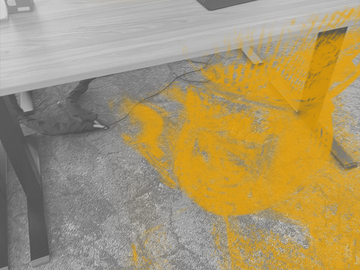
\includegraphics[width=\cw cm,height=\ch cm]{change_nor002.png}};
\draw[frm] (chi.south west) rectangle (chi.north east);
\node[img, anchor=north west, draw=white, line width=0.7pt] (chb) at ($(chi.north west)+(0.05,-0.05)$)
  {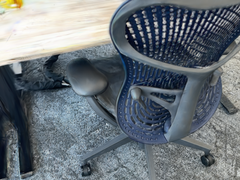
\includegraphics[width=0.76cm,height=0.57cm]{change_nor002_before.png}};
\node[lbl, anchor=south west, text=white, fill=black, fill opacity=0.55, text opacity=1, inner sep=0.6pt, font=\sixpt]
  at (chb.south west) {before};
\def\xCt{\xC+0.12+\cw+0.15}            % left edge of the text column
\node[lbl, anchor=west] at (\xCt, \yB-0.98) {$c=1-\cos(\R^{\old},\R^{\new})$};
\node[lbl, anchor=west] at (\xCt, \yB-1.43) {$\bar c$: min of the last $k{=}2$};
\node[lbl, anchor=west, text=chgtxt] at (\xCt, \yB-1.90) {fires if $\bar c>\theta(h)$};

% ================================================================== (8) reset and re-admission
\node[ttl, text=chgtxt] at (\xE,\yB) {\step{chg}{8} Reset, re-admission};
\node[lbl] at (\xE+\wE/2, \yB-0.82) {fired: sums restart from this view};
\node[lbl] at (\xE+\wE/2, \yB-1.32) {re-admit after $\nu\ge3$ views if the};
\node[lbl] at (\xE+\wE/2, \yB-1.76) {mean $\lvert d^{\mathrm{obs}}-d^{\mathrm{ctr}}\rvert\le5$\,cm};

% ================================================================== arrows
\draw[arr, black!75] (\xA+\wA, \ya) -- (\xB, \ya);
\draw[arr, black!75] (\xB+\wB, \ya) -- (\xC, \ya);
\draw[arr, black!75] (\xC+\wC, \ya) -- (\xD, \ya);
\draw[arr, black!75] (\xD+\wD, \ya) -- (\xE, \ya);
\draw[arr, black!75] (\xE+\wE, \ya) -- (\xF, \ya);
% the current view and the Gaussian's earlier evidence go into the test (right of its title)
\draw[chgarr] (\xC+\wC-0.18, -\hT) -- (\xC+\wC-0.18, \yB) node[midway, left, lbl, text=chgtxt, inner sep=1.5pt] {$\nu_v\uv_v$};
\draw[chgarr] (\xD+0.70, -\hT) -- (\xD+0.70, \yB) node[midway, right, lbl, text=chgtxt, inner sep=1.5pt] {$\R^{\old}$};
% threshold: mapping-pass scores in, theta(h) out
\draw[arr, black!55, line width=0.5pt] (\xC, \yB-1.20) -- (\xB+\wB, \yB-1.20);
\draw[chgarr] (\xB+\wB, \yB-1.75) -- (\xC, \yB-1.75);
% fired -> reset; reset -> sums; changed flag -> robust set
\draw[chgarr] (\xD+\wD, \yB-1.30) -- (\xE, \yB-1.30);
\draw[chgarr, line width=1.0pt, rounded corners=2pt] (\xE+0.40, \yB) -- (\xE+0.40, \yB+0.22) -- (\xD+\wD-0.40, \yB+0.22)
  -- (\xD+\wD-0.40, -\hT);
\node[lbl, text=chgtxt, anchor=west, inner sep=1pt, font=\scriptsize\bfseries] at (\xE+0.45, \yB+0.22) {reset};
\draw[chgarr] (\xE+\wE, \yB-1.30) -- (\xF, \yB-1.30);
% next keyframe
\draw[arr, black!55, dash pattern=on 2.2pt off 1.4pt] (\xE+\wE-0.30, 0) -- (\xE+\wE-0.30, 0.38)
  -- (\xA+\wA-0.35, 0.38) node[pos=0.5, above, lbl, text=black!70, inner sep=1pt] {next keyframe $v{+}1$}
  -- (\xA+\wA-0.35, 0);
\end{tikzpicture}
\end{document}
